\subsection{Two dimensional uniform dataset with holes}
\label{sec:2d-holes}

In order to test for the adaptability of the randomized SOM to different topologies, we created a two dimensional uniform dataset with holes of various size and at random positions (see figure \ref{fig:2D-holes:results}B). Such holes are known to pose difficulties to the regular SOM since neurons whose codewords are over a hole (or in the immediate vicinity) are attracted by neurons outside the holes from all sides. Those neurons hence become dead units that never win the competition. In the RSOM, this problem exists but is less severe thanks to the absence of regularity in the underlying neural topology and the loose constraints (we use 2 neighbors to build the topology). This can be observed in \ref{fig:2D-holes:results}B) where the number of dead units is rather small and some holes are totally devoid of any neurons. Furthermore, when a sample that does not belong to the original distribution is presented, it can be observed that the answer of the map is maximal for a few neurons only (see figure \ref{fig:2D-holes:results}G)).


%The second experiment is designed to investigate how the SOM algorithms cope with two-dimensional uniformly distributed data points with holes ($x_1, x_2 \sim \mathcal{U}(0, 1)$). Therefore, in this case the input to the maps is two-dimensional Euclidean points on a plane, where we put some holes at random places on the plane (see Figure~\ref{Fig:persistence_exp2b} {\bfseries \sffamily B}, blue discs). We train again both the VSOM and the Kohonen maps over $25000$ samples for $25000$ epochs and each map consists of $1024$ neurons. For the VSOM we define the topology of the map using a blue noise distribution (see Figure~\ref{Fig:experiment2b} {\bfseries \sffamily A}) and for the Kohonen we use the standard rectangular Euclidean grid. After convergence both algorithms generate proper topographic maps covering the  input space. Figure~\ref{Fig:experiment2b} {\bfseries \sffamily B} shows the mapping of VSOM learning algorithm (white discs and black segments) along with the input space (blue discs). We observe that not too many neurons cover the holes.

This observation is also supported by our topological analysis shown in figure \ref{fig:2D-holes:analysis}. Figures
\ref{fig:2D-holes:analysis}A, B, and C show the persistent barcodes where we can see the lifespan of each (birth, death)
pair (for more details about how we compute these diagrams see Section~\ref{sec:tda}). We observe that both the SOM and
the RSOM capture both the $H0$- and $H1$-homology of the input space, however the RSOM seems to have more persistent 
topological features for the $H1$-homology (orange lines). This means that the RSOM can capture more accurately the 
holes which are present in the input space. Roughly speaking we have about eight holes (see figure~\ref{fig:2D-holes:results}B) and we count about eight persistent features (the longest line segments
in the barcode diagrams) for RSOM in \ref{fig:2D-holes:analysis}C. On the other hand, the important persistent features
for the SOM are about five. In a similar way the persistent diagrams in figures~\ref{fig:2D-holes:analysis}C, D, and E
show that both RSOM and SOM capture in a similar way both the $H0$- and $H1$-homology features, although the 
RSOM (panel F) captures more holes as the isolated orange points away from the diagonal line indicate. This
is because the pairs that are further away from the diagonal are the most important meaning that they represent 
topological features that are the most persistent during the filtration process. 
Furthermore, we measure the Bottleneck distance between the persistence diagrams of input space and those of 
SOM and RSOM. The SOM's persistence diagram for $H0$ is closer to the input space (SOM: $0.000829$, RSOM: $0.001$),
while the RSOM's persistence diagram is closer to input's one for the $H1$ (SOM: $0.00478$, RSOM: $0.0037$). 
Finally, we ought to point out that the scale between panels A (D) and B, C (E, F) are not the same since the 
self-organization process has compressed information during mapping the input space to neural one.


% On the upper part of this figure, we can see that the 1-homology (or H1, blue segments, blue dots) are more elongated for RSOM (last column) when compared to the regular SOM (central column). These segments correspond to the lifespan of H1 features when the $\alpha$ radius is increased and we can observe that the RSOM is closer to the actual distribution (left column) when compared to SOM. More precisely, we observe that the number of holes in figure~\ref{fig:2D-holes:results} is eight. Furthermore, we notice that the number of persistent blue segments (first raw of figure~\ref{fig:2D-holes:analysis}) in persistent barcodes of figure~\ref{fig:2D-holes:analysis} is about eight for the input space and about the same for the RSOM. The regular SOM expresses less persistent blue segments. The length of the blue or red segments in the barcodes indicate the lifespan  of the filtration under the variation of radius $\alpha$. The more a segment survives the more important that topological feature is. Therefore, we can claim that the RSOM has about six persistent (significant) blue segments meaning that there are eight \emph{holes} in the corresponding neural space. On the contrary, regular SOM has less persistent segments of 1-homology (blue lines) implying that it covers more regularly the input space. Similar results are shown in the second raw of figure~\ref{fig:2D-holes:analysis}, where the persistent diagrams display the pairs (birth, death). Every time the radius $\alpha$ increases new pairs are born or die as we have already described in Section~\ref{sec:topo}. 


% However, 0-homology (H0, red segments) of RSOM and SOM behavior is very similar but also quite different from the actual distribution. 

% \npr{ Here, an explanation of what are the red lines would be necessary. Also, concerning H0, I'm not sure how to explain the difference with SOM, RSOM and the actual distribution and what does that mean.}

%Differences in $H0$ are attributed to the different neural space topology the two algorithms, the Kohonen and the VSOM, use. VSOM's neurons are placed not on an rectangular Euclidean grid as Kohonen's do, but instead on a random (following a blue noise distribution) Euclidean grid. 

% \npr{ Where is the referenced figure below? Where is the explanation concerning birht death rate on the analysis figure ?}


% In Figures~\ref{Fig:experiment2b} {\bfseries \sffamily C}-{\bfseries \sffamily H} we show the receptive fields of six randomly chosen units from the VSOM  map. We see that different stimuli are captured by different units implying that the topographic map of VSOM map is well-formed. 



\begin{figure}
  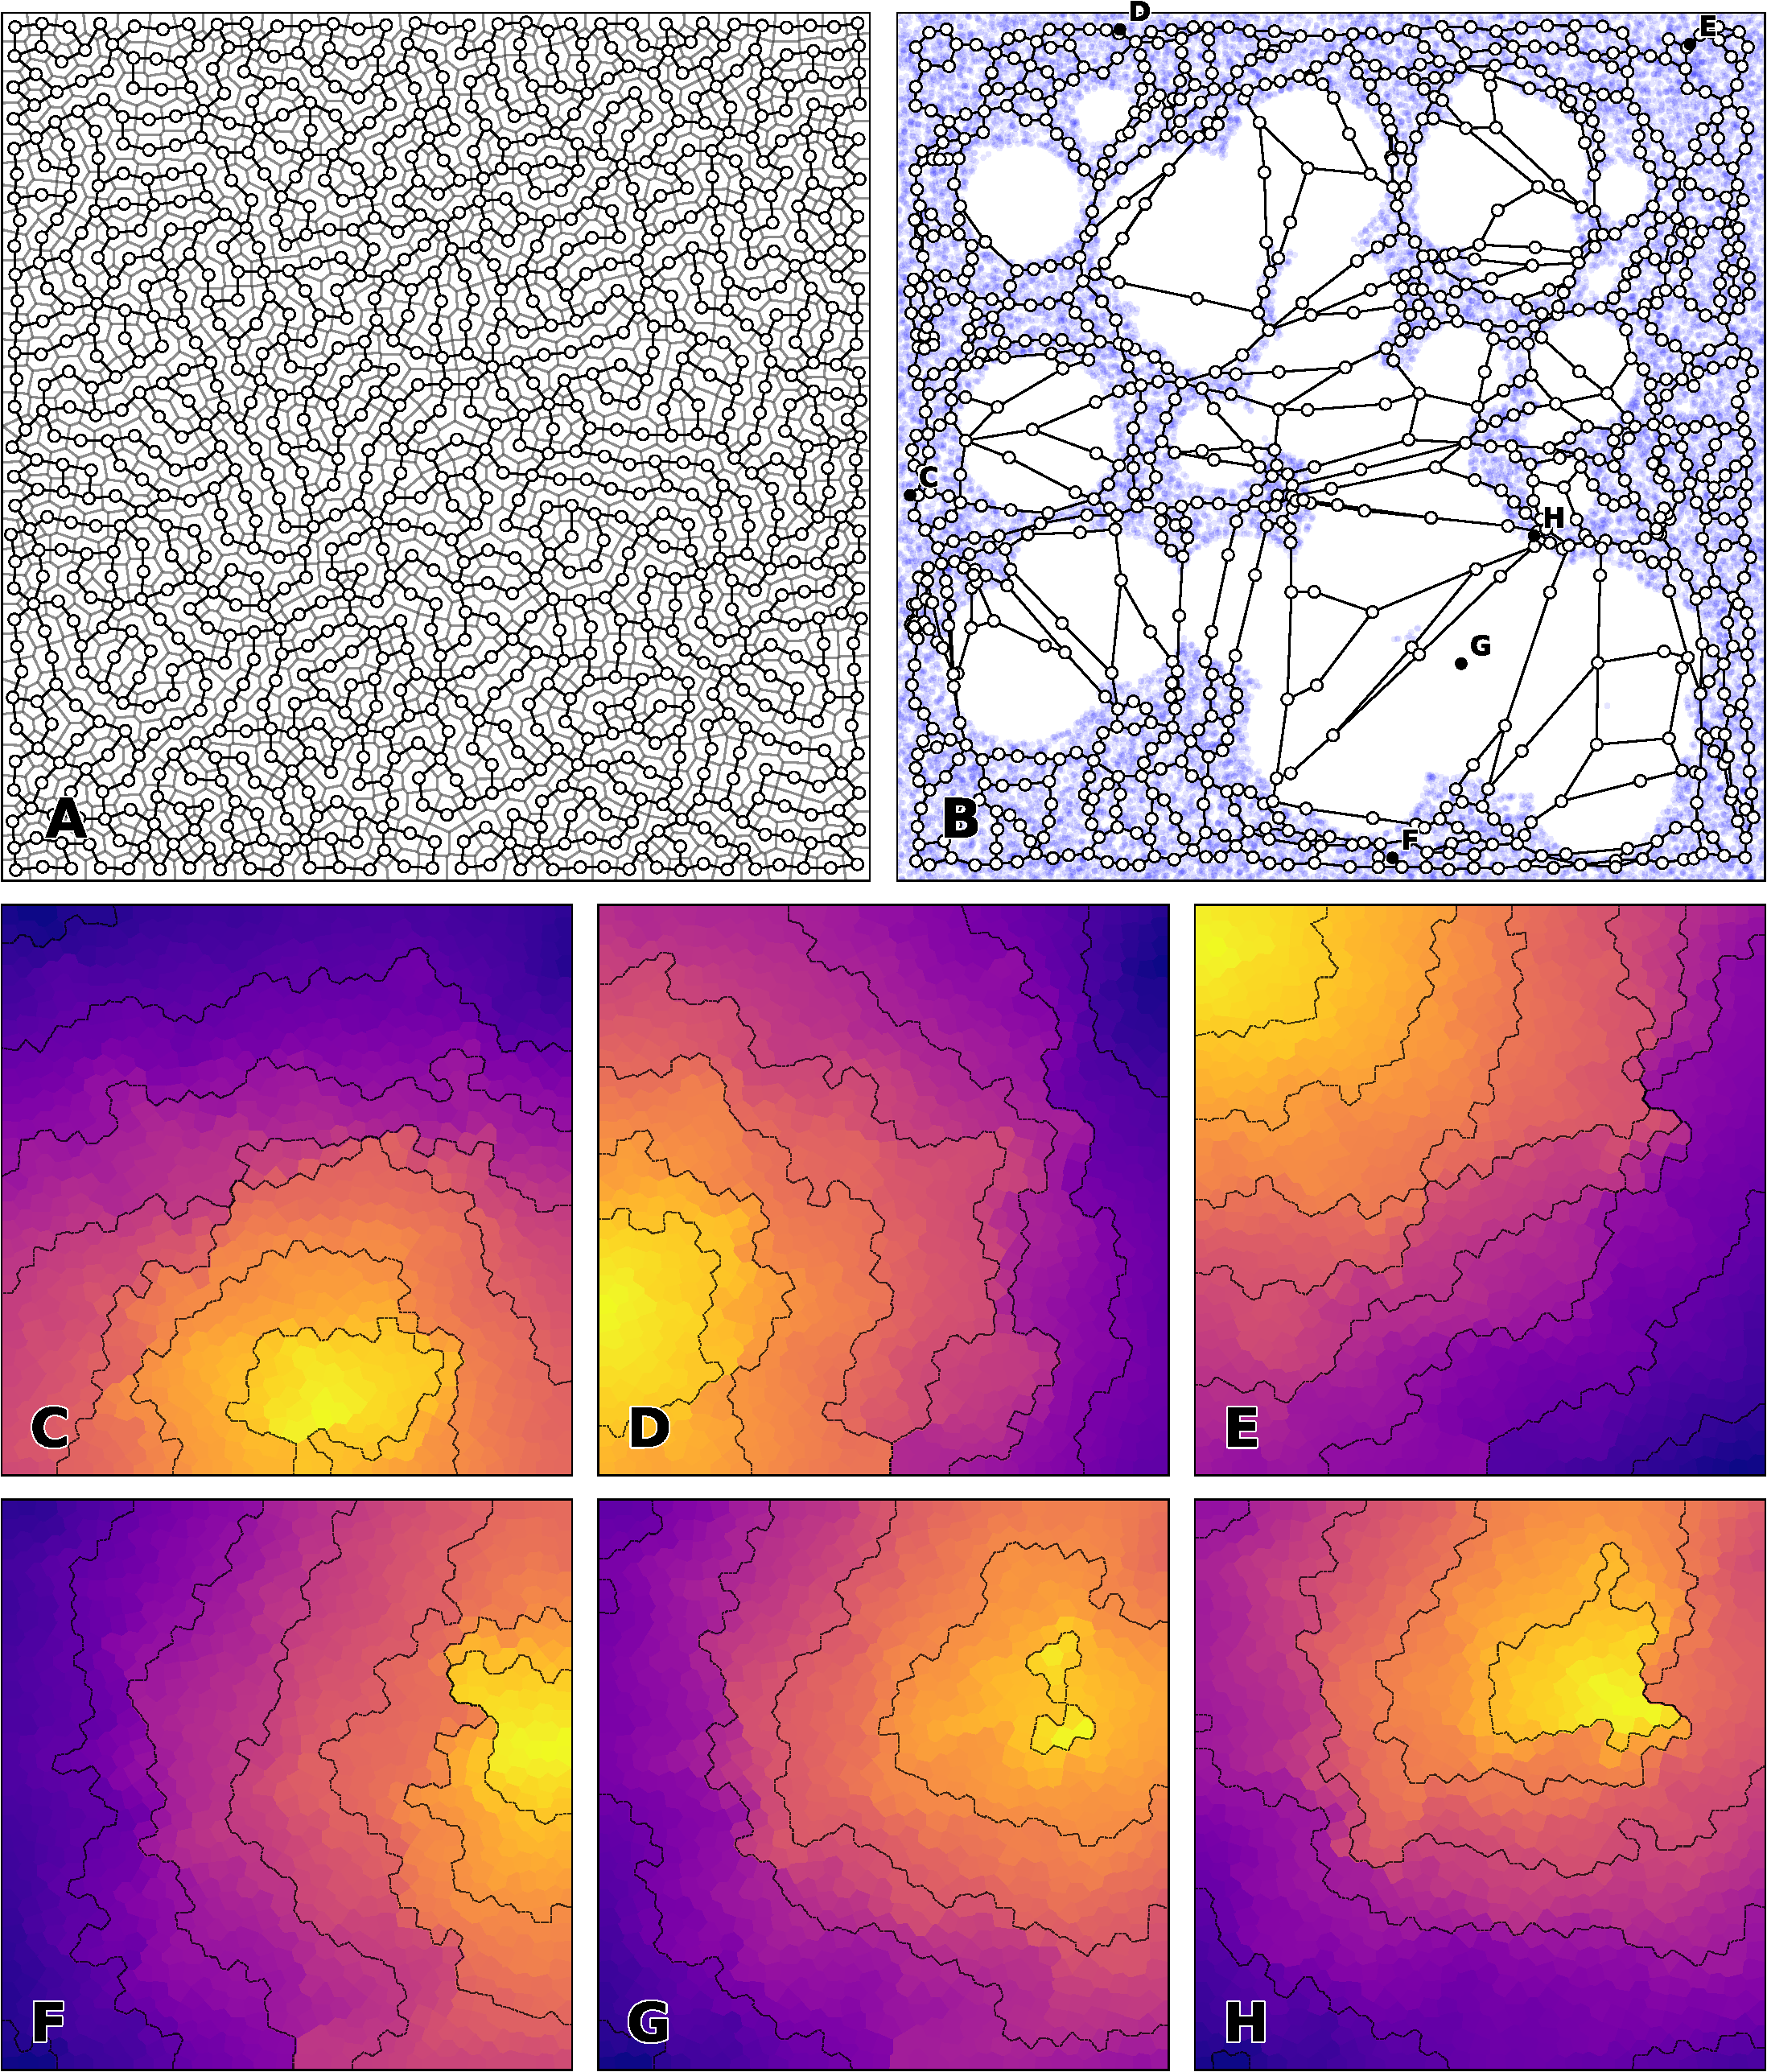
\includegraphics[width=\columnwidth]{experiment-2D-holes.pdf}
  \vspace{2mm}
  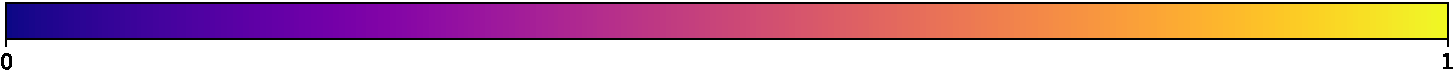
\includegraphics[width=\columnwidth]{figures/colormap.pdf}
  %
  \caption{%
  %
  {\bfseries \sffamily Two dimensional uniform dataset with holes (results)}
  %
  Randomized SOM made of $1024$ neurons with a $2$-nearest neighbors induced topology. Model has been trained for $25,000$ epochs on two-dimensional points drawn from a uniform distribution on the unit square with holes of various sizes and random positions. \textbf{A} Map topology in neural space. \textbf{B} Map topology in data space. \textbf{C to H} Normalized distance map for six random samples. The \textbf{G} point has been purposely set outside the point distribution. Normalization has been performed for each sample in order to enhance contrast but this prevents comparison between maps.
  %
  }
  \label{fig:2D-holes:results}
\end{figure}

\begin{figure}
  \centering
  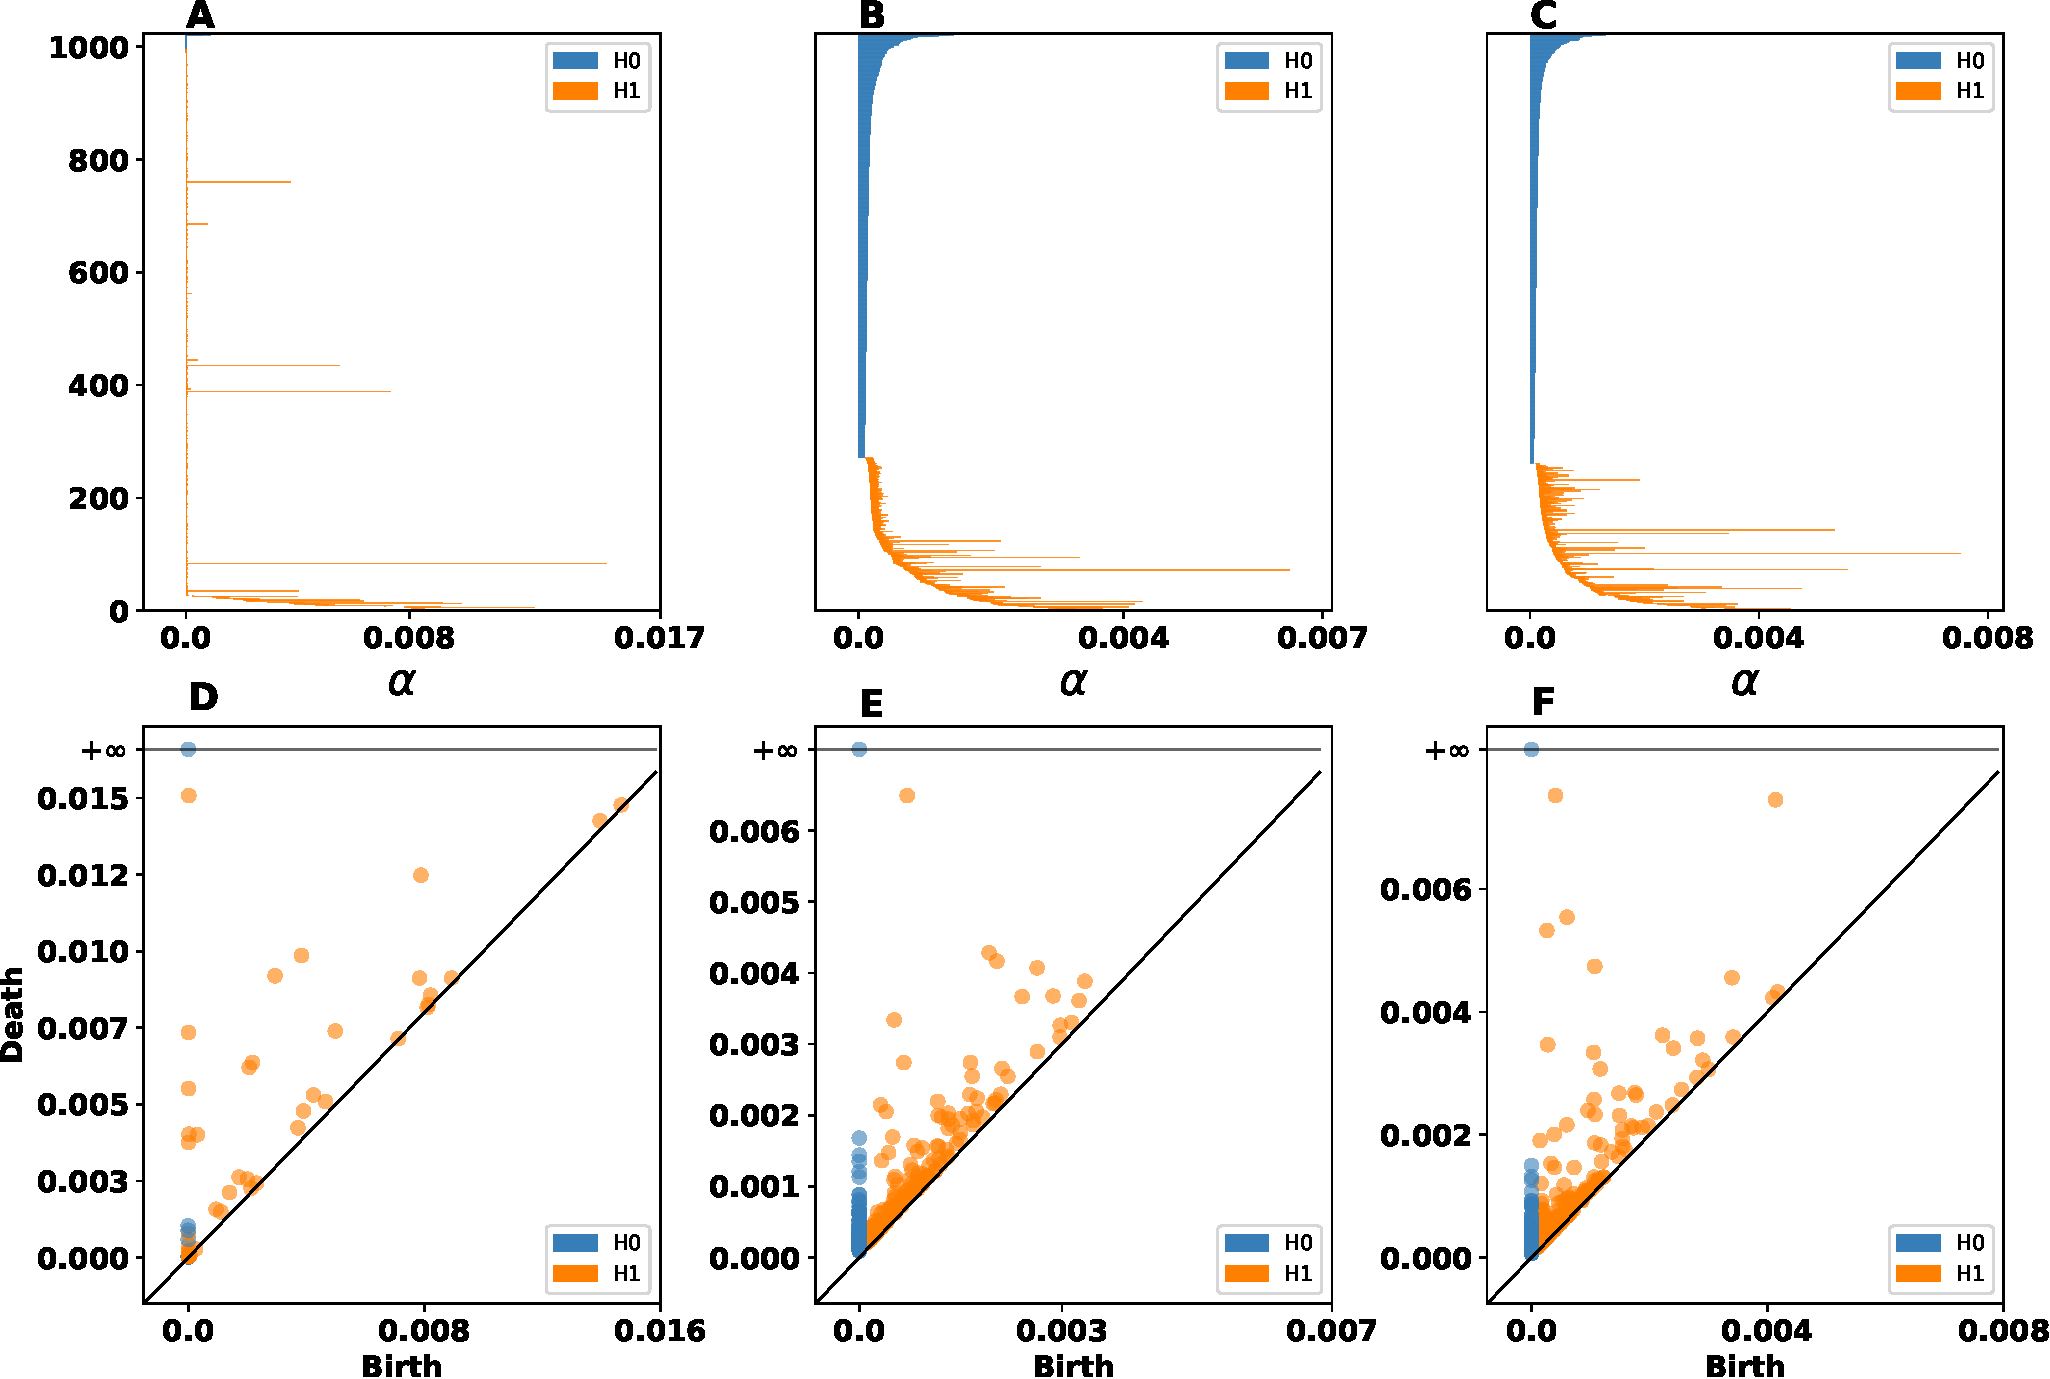
\includegraphics[width=\columnwidth]{experiment-2D-holes-analysis.pdf}
  %
  \caption{{\bfseries \sffamily Two dimensional uniform dataset with holes (analysis)}
  Persistent Barcodes of \textbf{A} input space, \textbf{B} SOM, and \textbf{RSOM}.
  The blue and orange line segments represent the $H0$- and $H1$-homology, respectively. This means
  that blue color represents connected segments within the space and orange color reflects the holes
  within the space. The longer the line segment the more important the corresponding topological
  feature. \textbf{D} illustrates the persistent diagram for the input space. \textbf{E} and \textbf{F}
  depict the persistent diagrams for SOM and RSOM, respectively. Again blue dots indicate $H0$-homology
  features and orange dots represent $H1$-homological features.}
  \label{fig:2D-holes:analysis}
\end{figure}
